\documentclass[11pt]{article}
\usepackage{listings}
\usepackage{graphicx}
\usepackage{color}
\usepackage{amsmath}

\definecolor{codegreen}{rgb}{0,0.6,0}
\definecolor{codegray}{rgb}{0.5,0.5,0.5}
\definecolor{codepurple}{rgb}{0.58,0,0.82}
\definecolor{backcolour}{rgb}{0.95,0.95,0.92}
 
\lstdefinestyle{mystyle}{
    backgroundcolor=\color{backcolour},   
    commentstyle=\color{codegreen},
    keywordstyle=\color{blue},
    numberstyle=\tiny\color{codegray},
    stringstyle=\color{codepurple},
    basicstyle=\footnotesize,
    breakatwhitespace=false,         
    breaklines=true,                 
    captionpos=b,                    
    keepspaces=true,                 
    numbers=left,                    
    numbersep=5pt,                  
    showspaces=false,                
    showstringspaces=false,
    showtabs=false,                  
    tabsize=2
}
 
\lstset{style=mystyle}

\begin{document}
\lstset{language=Matlab}

\title{COMPM012 - Coursework 3}
\author{Esben A. S\o rig}

\maketitle

\section{Practical}

\subsection{k-means implementation}
    \begin{lstlisting}
function [clusterings, centers] = mykmeans(X, k)
    % Randomly initialize centers of clusters
    c = datasample(X, k, 'Replace', false);
    r = repmat(0, size(X, 1), k);
    oldr = 1; % something that is not equal to r initially
    
    dist = @(x, y) norm(x-y);
    
    % Loop as long as the clustering is changing
    while ~isequal(r, oldr)
        oldr = r;
        
        % Assign points to clusters
        for i = 1:size(X,1)
            cluster = 1;
            for j = 1:k
                if dist(X(i, :), c(j, :)) <  dist(X(i, :), c(cluster, :))
                    cluster = j;
                end
            end

            r(i, :) = [repmat(0, 1, cluster-1) 1 repmat(0, 1, k-cluster)];
        end

        % Update center positions
        for i = 1:k
            npoints = 0;
            c(i, :) = 0;
            for j = 1:size(r, 1)
                c(i, :) = c(i, :) + r(j, i)*X(j, :);
                npoints = npoints + r(j, i);
            end
            c(i, :) = c(i, :)/npoints;
        end
    end
    
    centers = c;
    % Output formatting (vector with cluster index for each row in X)
    clustering = repmat(0, size(X,1), 1);
    for i = 1:size(X,1)
       for j = 1:k
           if r(i, j) == 1
                clustering(i) = j;
                break;
           end
       end
    end
   
    clusterings = clustering;
end\end{lstlisting}

\subsection{k-means test on data generated from three gaussians} Firstly, we generate the data and run the k-means algorithm on it.
    \begin{lstlisting}
% Generate data
data = genData2;

% Put data for each cluster in a seperate list
cluster1 = [];
cluster2 = [];
cluster3 = [];
[clusterings, centers] = mykmeans(data, 3);

for i = 1:size(data, 1)
    if clusterings(i) == 1
        cluster1 = [cluster1; data(i, :)];
    end
    if clusterings(i) == 2
        cluster2 = [cluster2; data(i, :)];
    end
    if clusterings(i) == 3
        cluster3 = [cluster3; data(i, :)];
    end
end\end{lstlisting}
    
    We can now plot the clusters the algorithm has found
    \begin{lstlisting}
figure
hold on

scatter(centers(:, 1), centers(:, 2), 200, 'xblack');
scatter(cluster1(:, 1), cluster1(:, 2));
scatter(cluster2(:, 1), cluster2(:, 2));
scatter(cluster3(:, 1), cluster3(:, 2));
legend('Centers', 'Cluster1', 'Cluster2', 'Cluster3');
hold off\end{lstlisting}
    
    \begin{center}
    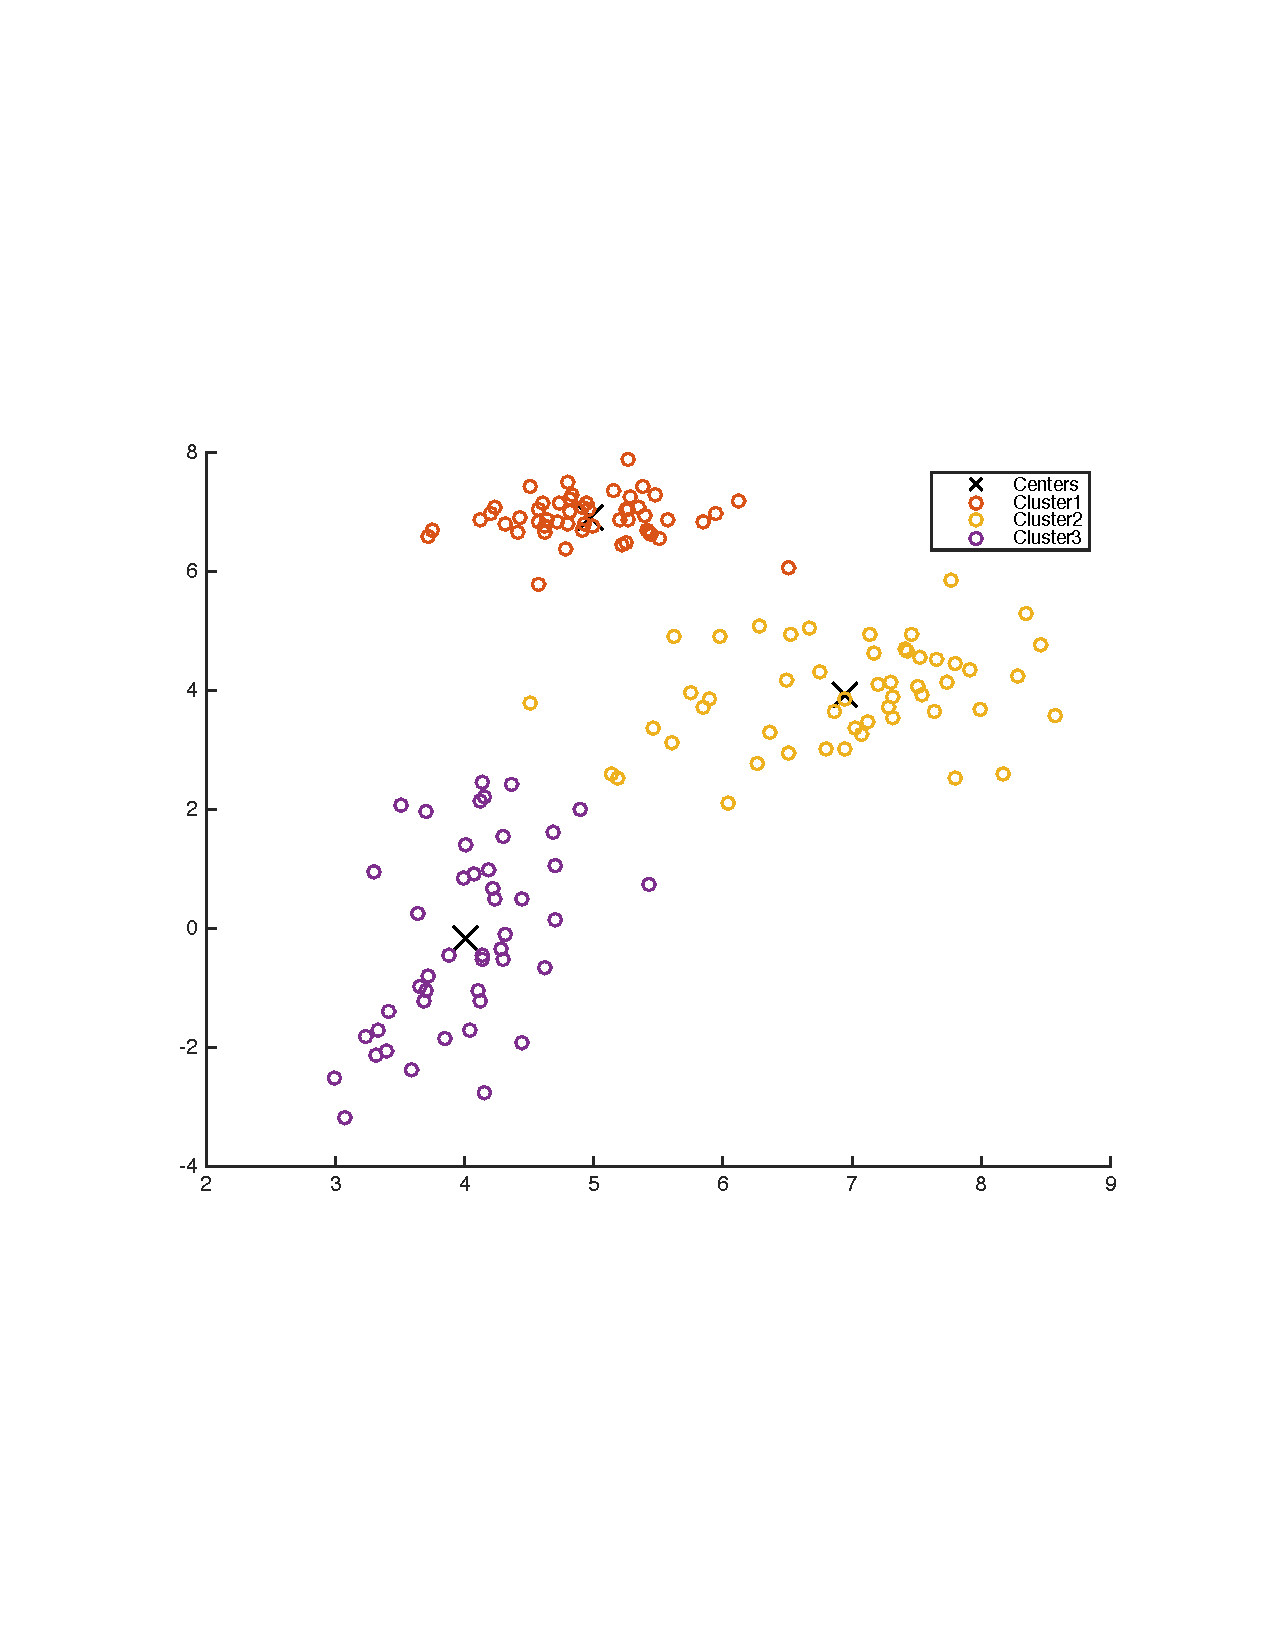
\includegraphics[width=\linewidth]{2-1}
    \end{center}

    
    Comparing this to the true classifications
    \begin{lstlisting}
figure
hold on
scatter(data(1:50, 1), data(1:50, 2));
scatter(data(51:100, 1), data(51:100, 2));
scatter(data(101:150, 1), data(101:150, 2));
legend('True Cluster1', 'True Cluster2', 'True Cluster3');
hold off\end{lstlisting}
    
    \begin{center}
    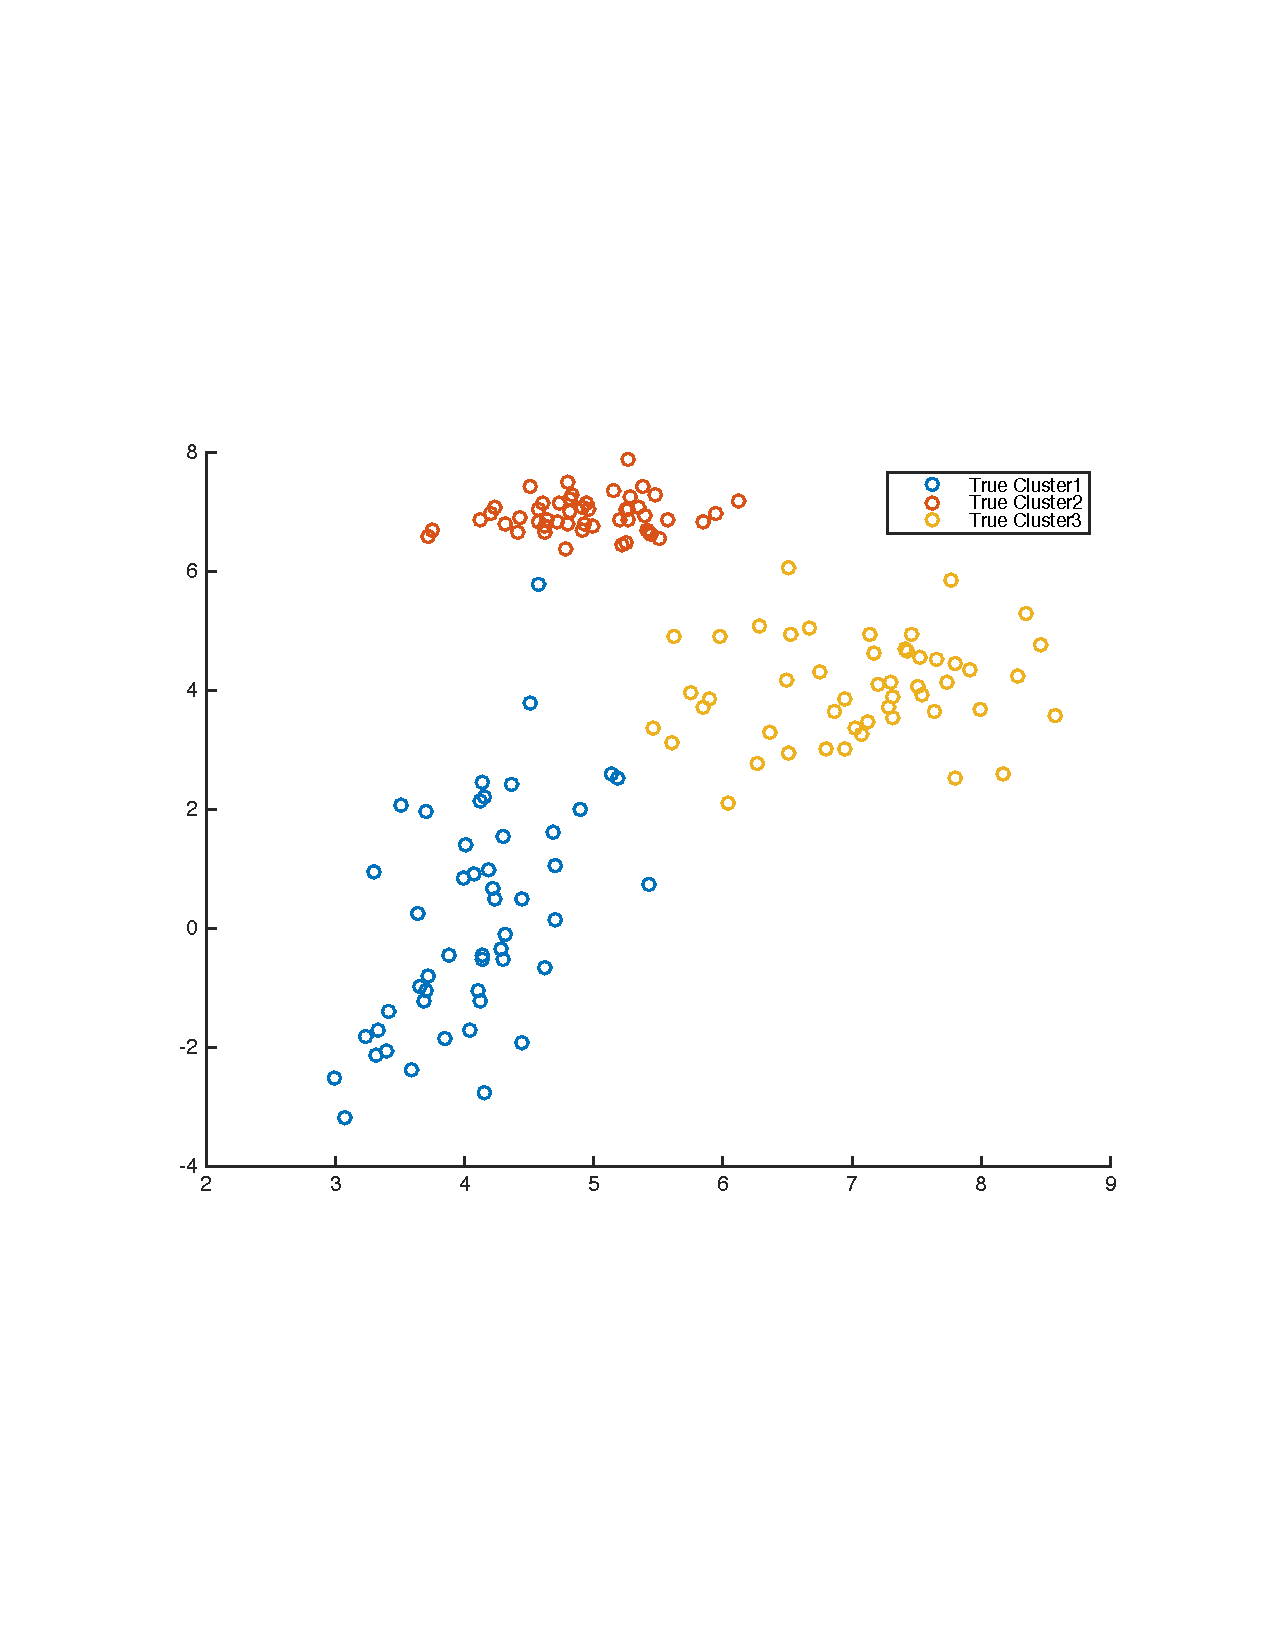
\includegraphics[width=\linewidth]{2-2}
    \end{center}
    
    We clearly get an intuition of how the k-means algorithm is performing on the data. Please see appendix \ref{appendix:movie} for the code that creates the animation of the convergence to a solution for this dataset.
    \par We measure the mean error and standard deviation of the error of the clustering over a 100 runs of the algorithm.
    \begin{lstlisting}
%% Error measurements
errors = [];
for j = 1:100
    [clusterings, centers] = mykmeans(data, 3);
    
    % keep track of the classifications of each true cluster
    firstcluster = [0,0,0];
    secondcluster = [0,0,0];
    thirdcluster = [0,0,0];
    for i = 1:50
        firstcluster(clusterings(i)) = 1 + firstcluster(clusterings(i));
    end
    for i = 51:100
        secondcluster(clusterings(i)) = 1 + secondcluster(clusterings(i));
    end
    for i = 101:150
        thirdcluster(clusterings(i)) = 1 + thirdcluster(clusterings(i));
    end
    % We assume that the mode of the classifications of a true cluster is the class of the true cluster. Therefore, the error of a cluster is the frequency of other classifications appearing for that cluster.
    firstcluster = sort(firstcluster);
    secondcluster = sort(secondcluster);
    thirdcluster = sort(thirdcluster);
    misclassifications = firstcluster(1) + firstcluster(2) + secondcluster(1) + secondcluster(2) + thirdcluster(1) + thirdcluster(2);
    errors = [errors misclassifications/150];
end

meanerror = mean(errors)
stddeviationerror = std(errors)\end{lstlisting}
    
    Which returns:
    \begin{lstlisting}
meanerror =
    0.1438
stddeviationerror =
    0.0155\end{lstlisting}

\section{Questions}
\subsection{Dataset with local minima} We can easily construct a dataset on which our k-means algorithm has local minima. An example of such a dataset is the set $\{ (0,0), (2,0), (-1, 4), (3, 4) \}$. This is clear if we plot the data.
    \begin{lstlisting}
X = [0, 0; 2,0; -1 4; 3 4];

hold on
axis([-2 5 -1 5]);
scatter(X(:, 1), X(:, 2));\end{lstlisting}
    Which gives the plot:
    \begin{center}
    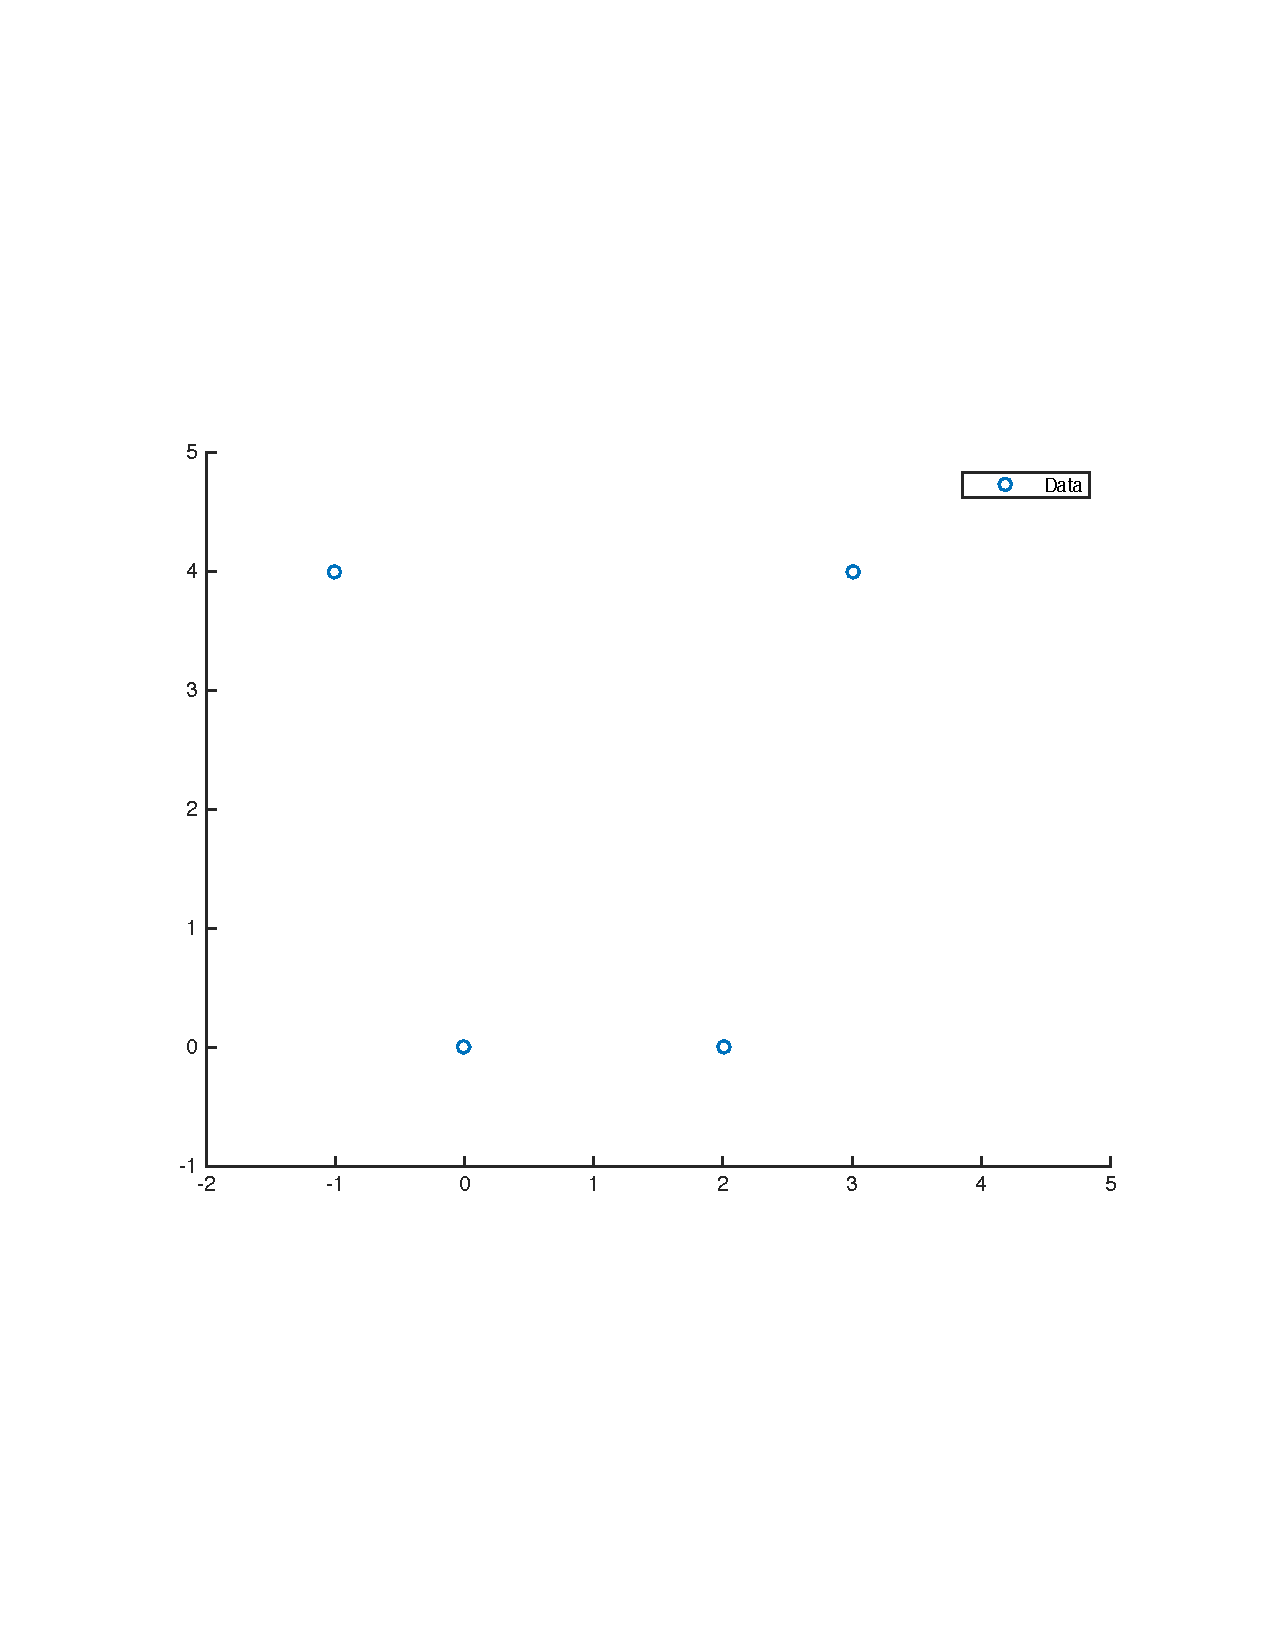
\includegraphics[width=\linewidth]{localminimapoints}
    \end{center}
    
    Running k-means on this dataset will converge in one of two local minima. We run the algorithm twice and plot the centers of the clusters: (in order to get two different results, this code may have to be run several times)
    
    \begin{lstlisting}
[clustering1, centers1] = mykmeans(X, 2);
[clustering2, centers2] = mykmeans(X, 2);
legend('Data');

scatter(centers1(:, 1), centers1(:, 2));
scatter(centers2(:, 1), centers2(:, 2));

legend('Data', 'Minimum 1 centers', 'Miinimum 2 centers');
hold off\end{lstlisting}

    Which produces:
    
    \begin{center}
    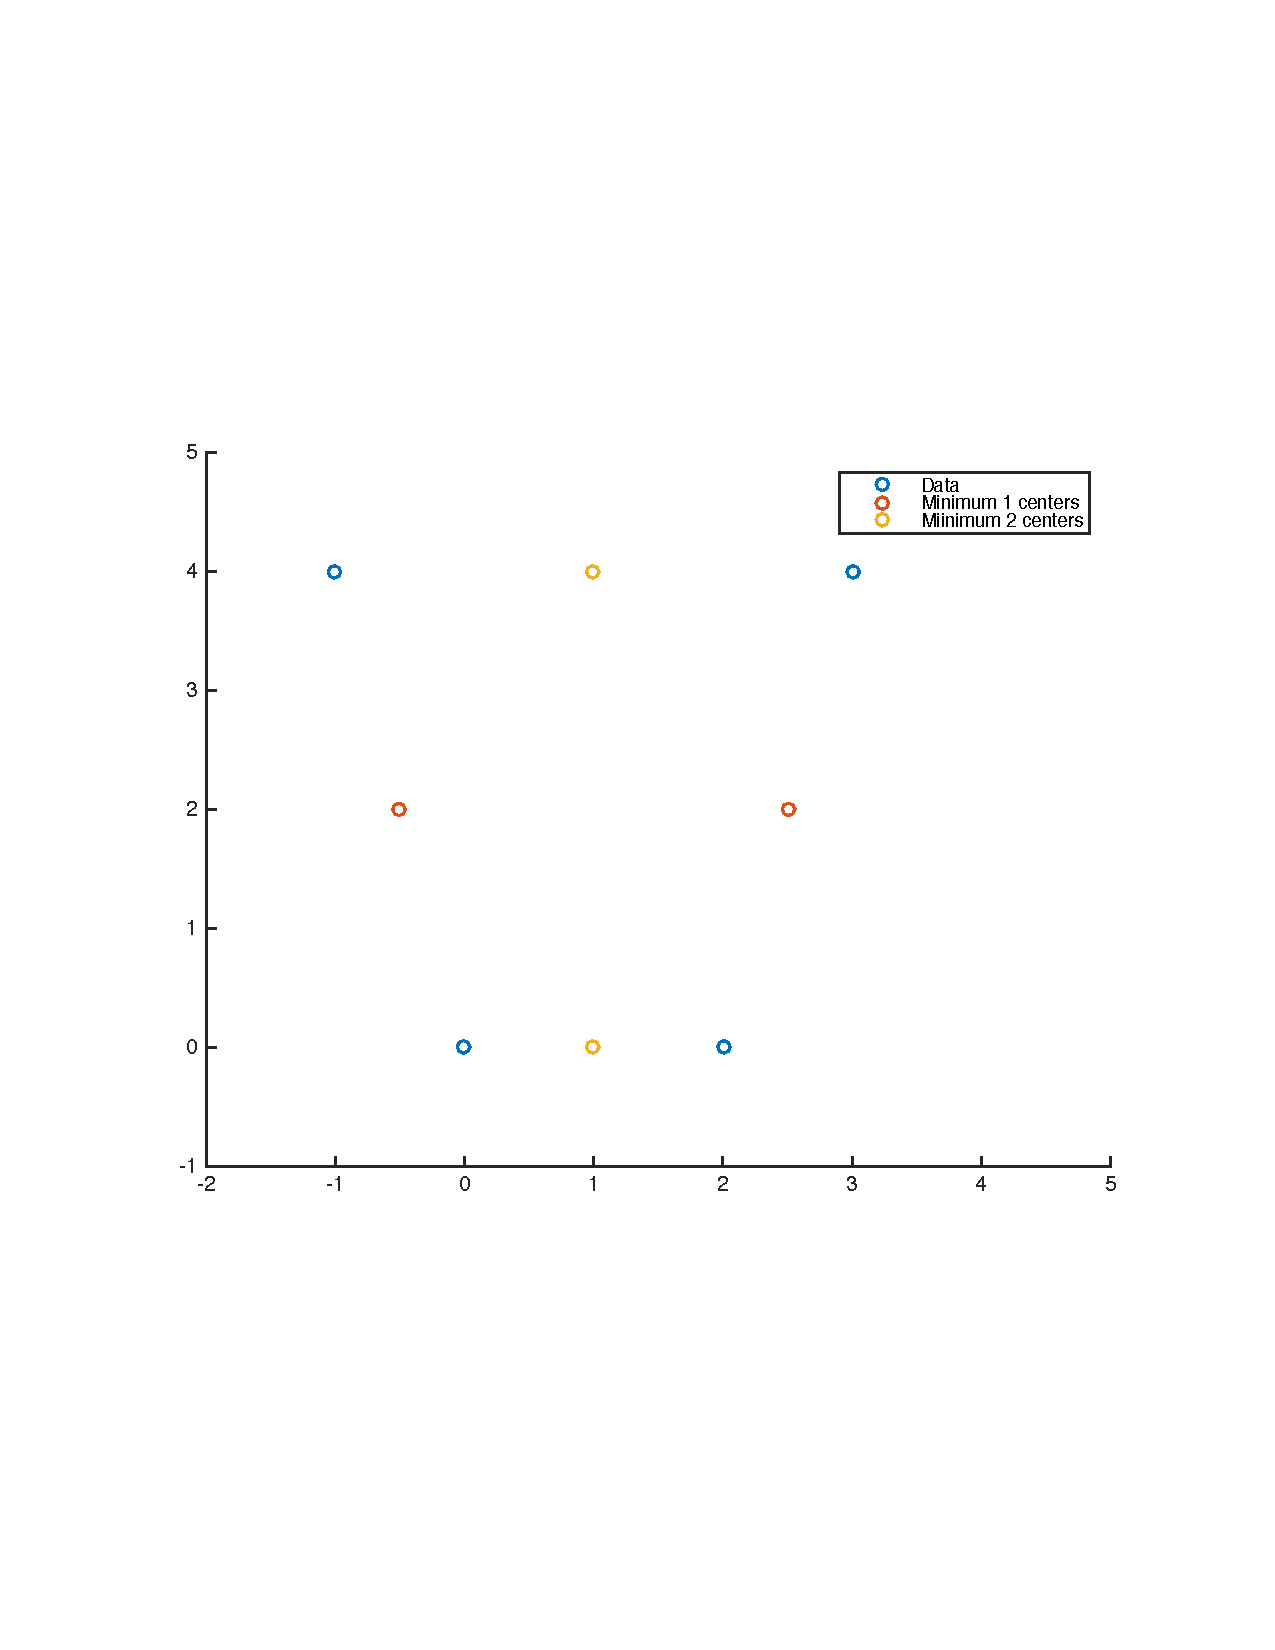
\includegraphics[width=\linewidth]{localminima}
    \end{center}
    
    Here we clearly see the two local minima of the convergence on the four data points.

\subsection{Argument that the centroid is the minimizer of the sum of squared distances}
    We can minimize the summed squared error
    
    \begin{equation}
        SSE = \sum_{i=1}^k \sum_{\mathbf{x} \in C_i} ||\mathbf{x} - \mathbf{c}_i||^2 
        = \sum_{i=1}^k \sum_{\mathbf{x} \in C_i} (\mathbf{x} - \mathbf{c}_i)^2
    \end{equation}
    
    for the $k^{th}$ centroid by setting the derivative with respect to the $k^{th}$ centroid equal to zero.
    
    \begin{equation}
    \begin{split}
        \frac{\delta}{\delta \mathbf{c}_k} \sum_{i=1}^k \sum_{\mathbf{x} \in C_i} (\mathbf{x} - \mathbf{c}_i)^2
        &= \sum_{i=1}^k \sum_{\mathbf{x} \in C_i}  \frac{\delta}{\delta \mathbf{c}_k} (\mathbf{x} - \mathbf{c}_i)^2\\
        &= \sum_{\mathbf{x} \in C_k} 2(\mathbf{x}_k - \mathbf{c}_k) = 0\\
        \implies \sum_{\mathbf{x} \in C_k} \mathbf{c}_k &= \sum_{\mathbf{x} \in C_k} \mathbf{x}_k\\
        \implies \mathbf{c}_k &= \frac{1}{\sum_{\mathbf{x} \in C_k} 1} \sum_{\mathbf{x} \in C_k} \mathbf{x}_k
    \end{split}
    \end{equation}
    
    We see that the minimizer of $\mathbf{c}_k$ is equivalent to the centroid of the cluster.
    
\subsection{Proof of convergence in finite amount of steps}

\section{Extension}
\subsection{k-means segmentation}

\subsection{(p, k)-means}

\section{Appendix}
    \subsection{Movie generation code} \label{appendix:movie}
        \begin{lstlisting}
%% Movie
X = data;
k = 3;
% Randomly initialize centers of clusters
c = datasample(X, k, 'Replace', false);
r = repmat(0, size(X, 1), k);
oldr = 1; % something that is not equal to r initially
movie = [];

dist = @(x, y) norm(x-y);

% Loop as long as the clustering is changing
while ~isequal(r, oldr)
    oldr = r;
    
    % Assign points to clusters
    for i = 1:size(X,1)
        cluster = 1;
        for j = 1:k
            if dist(X(i, :), c(j, :)) <  dist(X(i, :), c(cluster, :))
                cluster = j;
            end
        end

        r(i, :) = [repmat(0, 1, cluster-1) 1 repmat(0, 1, k-cluster)];
    end
    
    %MOVIE GENERATION
    % Split the data into the three clusters
    cluster1 = [];
    cluster2 = [];
    cluster3 = [];

    for i = 1:size(X, 1)
        if r(i,1) == 1
            cluster1 = [cluster1; X(i, :)];
        end
        if r(i,2) == 1
            cluster2 = [cluster2; X(i, :)];
        end
        if r(i,3) == 1
            cluster3 = [cluster3; X(i, :)];
        end
    end
    
    % Plot the centers and the three clusters
    hold on
    scatter(c(:, 1), c(:, 2), 200, 'xblack');
    if size(cluster1, 1) ~= 0
        scatter(cluster1(:, 1), cluster1(:, 2));
    end
    if size(cluster2, 1) ~= 0
        scatter(cluster2(:, 1), cluster2(:, 2));
    end
    if size(cluster3, 1) ~= 0
        scatter(cluster3(:, 1), cluster3(:, 2));
    end
    legend('Centers', 'Cluster1', 'Cluster2', 'Cluster3');
    hold off
    movie = [movie getframe];
    clf;
    % MOVIE GENERATION OVER

    % Update center positions
    for i = 1:k
        npoints = 0;
        c(i, :) = 0;
        for j = 1:size(r, 1)
            c(i, :) = c(i, :) + r(j, i)*X(j, :);
            npoints = npoints + r(j, i);
        end
        c(i, :) = c(i, :)/npoints;
    end
end
movie2avi(movie, 'k-means.avi', 'fps', 1);\end{lstlisting}





\end{document}
